\subsection{Cyclic Extensions}\label{sec_cyclic}

The aim of this subsection is to give a complete analysis of the case when $F/K$ is a cyclic extension of number fields. We show that for any $d\geq 2$ and representation $\rho$ of $C_d$, the product \eqref{eqn_localprod} of local factors is the norm of any quadratic subfield of $\QQ(\rho)$. 
%We also provide an exhaustive list of cases when the product may not be a norm of quadratic subfield of $\QQ(\rho)$. 
Firstly, we recall the following result, whose proof was covered in Example \ref{cyclic-relns}.

\begin{lemma}\label{lem_relation}
    Let $\rho$ be a representation of the cyclic group $C_d$. Then there is one unique relation $\Theta_\rho\in B(C_d)$ such that 
    $$\CC[C_d/\Theta_{\rho}]=\repnorm{\rho}=\bigoplus_{\fg\in\Gal(\QQ(\rho)/\QQ)}\rho^{\fg}.$$
    In particular, if $\rho=\psi_d$ is a faithful character of $C_d$, then
    $$\Theta_{\psi_d}=\sum_{k\mid d}\mu(k)C_k.$$
\end{lemma}


%We also the following definition that characterises those $d$ that always give norms of the quadratic subfields and those that do not. Recall that given some integer $d\geq 2$, $\rad(d)=\prod_{p\mid d}p$ is the smallest squarefree integer dividing $d$.

%\begin{defn}
    %Let $d\geq 2$ be an integer. We say that $d$ is \textbf{bad} if either $\rad(d)=2$ or $\rad(d)=6$ and $4\mid d$. Otherwise, we say that $d$ is \textbf{good}.
%\end{defn}

The main result of this section is to prove that for any $d$ and any representation $\rho$ od $C_d$, the product of local factors of an elliptic curve over $\QQ$ always gives a norm of any quadratic subfield of $\QQ(\rho)$.

\begin{thm}\label{thm_consistent_cyclic}
    Let $d\geq2$ be a positive integer and let $F/K$ be a Galois extension of number fields such that $\Gal(F/K)=C_d$. Let $\rho$ be a representation of $C_d$ and let $\Theta_\rho\in B(C_d)$ be such that
    $$\CC[G/\Theta_\rho]=\repnorm{\rho}.$$

    If $E/\QQ$ is a semistable elliptic curve at $2$ and $3$, then for any $\QQ(\sqrt{D})\subseteq\QQ(\rho)$,
    $$C(\Theta_\rho)\in N_{\QQ(\sqrt{D})/\QQ}(\QQ(\sqrt{D})^{\times}).$$
\end{thm}

The first step towards proving this theorem is to show that if the theorem holds for faithful characters, then it holds for arbitrary representations. 

\begin{lemma}
    Suppose that Theorem \ref{thm_consistent_cyclic} holds for faithful characters $\psi_d$. Then it also holds for any representation $\rho$ of $C_d$.
\end{lemma}
\begin{proof}
    Firstly, we show that the theorem also holds for arbitrary characters of $C_d$. Let $\psi_{d'}$ be a character of $C_d$ of order $d'$ for some $d'\mid d$, and recall that 
    $$\Theta_{\psi_{d'}}=\sum_{k\mid d'}\mu(k)C_{dk/d'}.$$ Since $\ker\psi_{d'}=C_{d/d'}$, we can view $\psi_{d'}$ as a faithful character of $C_{d'}$. Then the result follows immediately from the theorem applied to ${d'}$ and the $C_{d'}$-extension $F/F^{C_{d'}}$.
    Now assume that $\rho$ is any representation of $C_d$. Then $\repnorm{\rho}$ is a rational valued representation, and the representations
    $$\chi_k:=\repnorm{\psi_k}$$
    for each $k\mid d$ are a basis of the rational representations. Hence, there is a unique decomposition
    $$\repnorm{\rho}=\sum_{k\mid d}a_k\chi_k,\ a_k\in\ZZ,$$
    where
    which in particular implies that 
    $$C(\Theta_\rho)=\prod_{k\mid d}C(\Theta_{\psi_k})^{a_k}\equiv \prod_{\substack{k\mid d \\ a_k\text{ odd}} }C(\Theta_{\psi_k})^{a_k}\pmod{\QQss}.$$
    In Proposition \ref{index-fn-trivial} we showed that if $\QQ(\rho)\nsubseteq \QQ(\zeta_d)=\QQ(\psi_k)$, then $a_k$ was even, so if $a_k$ is odd, then $\QQ(\rho)\subseteq\QQ(\zeta_k)$. If $\QQ(\sqrt{D})$ is a quadratic subfield of $\QQ(\rho)$, then $C(\Theta_{\psi_k})$ is a norm from $\QQ(\sqrt{D})$ whenever $a_k$ is odd. This implies that $C(\Theta_\rho)$ is a norm from $\QQ(\sqrt{D})$ too, and thus Theorem \ref{thm_consistent_cyclic} holds.
\end{proof}

This lemma has the great advantage that it allows us to restrict our attention to faithful characters of $C_d$. To simplify notatation, we will denote $\Theta_d=\sum_{k\mid d}\mu(k)C_k\in B(C_d)$ as the $\psi_d$-relation, where $\psi_d$ is a faithful character of $C_d$.

\begin{rem}\label{rem_radical}
    Lemma \ref{lem_relation} has an important consequence. Given an integer $d\geq2$, note that a subgroup $C_k$ appears in $\Theta_d$ if and only if $C_k\leq C_{\rad(d)}$. Consequently, in terms of fields, if $L_k=F^{C_{d/k}}$ is the unique intermediate field with $[L_k:\QQ]=k$ for each $k\mid d$, then $C(\Theta_d)$ contains the local factors of $L_k$ if and only if $L_{d/\rad(d)}\subseteq L_k\subseteq F$.

    Following this observation, we will compute $T(\Theta_d)$ and $D(\Theta_d)$ by computing locally $\Tp(\Theta_d)$ and $\Tp(\Theta_d)$ for each prime $\pp$ of some conveniently chosen subfield $L_k\subseteq L_{d/\rad(d)}$, and then combinining this local information via the formula
    \begin{equation}\label{eqn_local_contr}
        T(\Theta_d)=\prod_{\pp}\Tp(\Theta_d)=\prod_\pp\left(\prod_{k\mid d} \Tp(C_k)^{\mu(k)}\right),    
    \end{equation}
    and where the same equation holds for $D(\Theta_d)$.
\end{rem}

To compute $\Tp(\Theta_d)$ for multiplicative reduction, the following notation will also be useful.

\begin{notation}\label{not_n}
    Let $n$ be a positive integer. Let 
    \[
        \tilde{n}=
        \begin{cases}
            1 \text{ if } n \text{ is odd,}\\
            2 \text{ if } n \text{ is even.}
        \end{cases}
    \]
\end{notation}
Therefore, if $E$ is an elliptic curve with multiplicative reduction at some prime $\pp$ of $K$ and $n=\nu_\pp(\Delta_{E,\pp}^{\min})$, then $c_\pp(E/K)=n$ if the reduction is split and $c_\pp(E/K)=\tilde{n}$ if non-split.

We divide the proof of Theorem \ref{thm_consistent_cyclic} for faithful characters into two separate cases: odd and even cyclic extensions. The main idea in both cases is to simplify the general case into smaller cases where we can directly compute $\Cp(\Theta_d)$ for each finite place $\pp$ of $K$. Unless stated otherwise, we assume thoughout that $$\Theta_d=\sum_{k\mid d}\mu(k)C_k\in B(C_d).$$





\subsubsection{Odd Cyclic Extensions} \label{case_Cp}

For the first case, we assume that $d$ is odd. Following the observation in Remark \ref{rem_radical}, we will calculate $\Cp(\Theta_d)$ for each finite place $\pp$ of some subfield of $F^{C_{\rad(d)}}$. However, before we calculate these terms explicitly for distinct cases, we prove a technical result that considerably simplifies the calculations of $\Dp(\Theta_d)$.

\begin{lemma}
    Let $q$ be an odd prime and $L/K$ a Galois extension of number fields such that $\Gal(L/K)=C_q$, and let $\pp$ be a prime in $K$. Let $E/\QQ$ be an elliptic curve and $\Theta_q=C_1-C_q\in B(C_q)$. Then by changing the model of $E$ over $K$, and therefore by rescaling the discriminat of $E$, $\Dp(\Theta_q)$ does not change up to squares.
\end{lemma}
\begin{proof}
    Let $\Delta_E,\Delta_E'$ be the discrimiants of two models of $E$ over $K$, and let $\lambda=(\Delta_E'/\Delta_E)^{1/12}\in K$. Write $\Dp'(\Theta_q)$ and $\Dp(\Theta_q)$ for the value usual terms using $\Delta_E$ and $\Delta_E'$ as discriminants, respectively. Then a simple calculation shows that
    
    $$\Dp(\Theta_q)=\frac{\prod_{\fP\mid\fp}|\lambda|_\fP}{|\lambda|_\pp}\Dp'(\Theta_q).$$
    Hence, the result will follow by showing that $\prod_{\fP\mid\fp}|\lambda|_\fP/|\lambda|_\pp\in\QQss$. 
    
    There are three cases, depending on the splitting behaviour of $\pp$ in $F$. 
    \begin{itemize}
        \item If $\pp$ splits, then there are $q$ primes above $\pp$ with the same residue field and normalized valuation. Hence $\prod_{\fP\mid\fp}|\lambda|_\fP=|\lambda|_\pp^q$.
        \item If $\pp$ is inert, then there is one prime $\fP$ above $\pp$ whose residue field is a degree $q$ extension and with the same normalized valuation. Hence $|\lambda|_\fP=|\lambda|_\pp^q$.
        \item If $\pp$ ramifies, then there is one prime $\fP$ above $\pp$, with equal residue field but with normalized valuation satisfying $\nu_\fP(\lambda)=q\mu_\pp(\lambda)$. Hence $|\lambda|_\fP=|\lambda|_\pp^q$ too.
    \end{itemize}
    Hence, we always have that 
    $$\frac{\prod_{\fP\mid\fp}|\lambda|_\fP}{|\lambda|_\pp}=|\lambda|_\pp^{q-1}\in\QQss$$
\end{proof}

The great advantage of this result is that once a prime $\pp$ has been chosen in some subfield of $F^{C_{\rad(d)}}$, we will be able to assume that $\Delta_E=\Delta_{E,\pp}^{\min}$. 

To prove Theorem \ref{thm_consistent_cyclic} for odd $d$, we first calculate $\Cp(\Theta_d)$ for simple cases, and then we use them to prove the general case. The following lemmas build on this idea.

\begin{lemma}\label{lem_Cp}
    Let $q$ be an odd rational prime, $F/K$ a Galois extension of number fields such that $\Gal(F/K)=C_q$ and $E/\QQ$ an elliptic curve with semistable reduction at $2$ and $3$. If $\Theta_q=C_1-C_q$, then 
    $$C(\Theta_q)=\frac{C_{E/F}}{C_{E/K}}$$
    is a norm from $\QQ(\sqrt{q^*})$.
\end{lemma}

\begin{proof}
    Fix some prime $\pp$ in $K$, and assume that $\Delta_E=\Delta_{E,\pp}^{\min}$. We calculate $\Cp(\Theta_q)$ depending on the reduction type of $\pp$. Primes $\pp$ of good reduction yield no non-trivial factors since $\Tp(\Theta_q)=\Dp(\Theta_q)=1$. Hence, we may only consider from now on primes of bad reduction. We also note since the extension $L/K$ is cyclic, the splitting behaviour of $\pp$ in $L$ is determined by the ramification index $e_\pp$ and the residual degree $f_\pp$. 
    
    If $\pp$ has multiplicative reduction, then $D_{\fP\mid\pp}(\Theta_q)=1$ and Table \ref{table_Cp} records $T_{\fP\mid\pp}(\Theta_q)$ depending on $e_\pp$ and $f_\pp$, where and the entries for split and non-split multiplicative reduction of type $\mathrm{I}_n$ are separated by a ``;''. To complete these calculations, we use repeatedly Proposition \ref{prop_semi_red} and Lemmas \ref{lem_mult_tam} and \ref{lem_add_tam}. We also use Notation \ref{not_n}.

    \begin{table}[!ht]
        \centering
        \begin{tabular}{|l|l|l|l|l|}
        \hline
        $e_\pp$ & $f_\pp$  & $T_{\fP\mid \pp}(C_q)$ & $T_{\fP\mid \pp}(C_1)$  & $\Tp(\Theta_q)$ \\ \hline
        $1$ & $1$ & $n;\tilde{n}$ & $n^q;\tilde{n}^q$ & $\square$ \\ \hline
        $q$ & $1$ & $n;\tilde{n}$ & $qn;\tilde{n}$ & $q\square;\square$ \\ \hline
        $1$ & $q$ & $n;\tilde{n}$ & $n;\tilde{n}$ & $\square$ \\ \hline
        \end{tabular}
        \caption{Contribution of semistable reduction primes in a $C_q$ extension.}
        \label{table_Cp}
    \end{table}

    Since $q$ is indeed a norm from $\QQ(\sqrt{q^*})$ by Lemma \ref{p-norm}, it follows that $\Tp(\Theta_q)$ is a norm from $\QQ(\sqrt{q^*})$ as well.

    Now assume $\pp$ has additive reduction, and let $p\ZZ=\pp\cap\QQ$. By assumption, $p\neq2,3$. We note that $D_{\fP\mid\pp}(\Theta_q)=1$ unless $\pp$ ramifies in $F/K$, and in that case it is a power of $N_{K/\QQ}(\pp)=p^s$. If $s$ is even, then $D_{\fP\mid\pp}(\Theta_q)\in\QQss$, so assume instead that $s$ is odd. If $L_\fP/K_\pp$ is wildly ramified, then $p=q$ is a norm from $\QQ(\sqrt{q^*})$. If $L_\fP/K_\pp$ is tamely ramified, then by Proposition \ref{prop_totally_ramified}, it follows that $q\mid p^s-1$ and therefore 
    \begin{equation}
        \left(\frac{q^*}{p}\right)=\left(\frac{p}{q}\right)=\left(\frac{p^s}{q}\right)=1
    \end{equation}
    Therefore, $p$ splits in $\QQ(\sqrt{q^*})$ and by Corollary \ref{cor_psplit_pnorm}, it follows that $p$ is a norm from $\QQ(\sqrt{q^*})$. 
    
    Finally, we compute $\Tp(\Theta_q)$. Note that since $q$ is odd, any inertia degree is odd and therefore if $\fP$ is any prime in $F$ above $\pp$, $\sqrt{D}\in K_\pp$ if and only if $\sqrt{D}\in L_\fP$ for any $D\in\QQ$. Moreover, if $q\neq 3$, then $\gcd(e_{\fP\mid\pp},12)=1$ and by Lemma \ref{lem_add_tam}, $c_\pp(E/K)=c_\fP(E/F)$. This implies that $$\Tp(\Theta_q)=c_\pp(E/K)^{\#\{\fP\mid\pp\}-1}\in\QQss$$ since the number of primes $\fP$ in $L$ above $\fp$ is odd. If $q=3$ and $\pp$ is unramified in $L/K$, then $e_{\fP\mid\pp}=1$ and the same reasoning shows that $\Tp(\Theta_q)=1$. Hence, assume $L_\fP/K_\pp$ is ramified and let $n=\nu_\pp(\Delta_{E,\pp}^{\min})$ be the valuation of the minimal discriminant of $E$ at $\pp$. By Lemma \ref{lem_add_tam}, we can obtain factors of $2$ and $3$. Since $3$ is a norm from $\QQ(\sqrt{-3})$, we only need to take care of the factors of $2$, which can only arise if $F_\fP/K_\pp$ is ramified, $\gcd(n,12)=2$ and $\sqrt{\Delta}\not\in K_\pp$. However, Lemma \ref{lem_nottwo} shows that these conditions cannot arise, and therefore $\Tp(\Theta_q)$ is a norm from $\QQ(\sqrt{-3})$ as desired.
\end{proof}

Next, we prove an analogous result for $C_{qr}$ extensions, where $q$ and $r$ are distinct odd rational primes.

\begin{lemma}\label{lem_Cpq}
    Let $q,r$ be distinct, odd rational primes and let $F/K$ be a Galois extension of number fields such that $\Gal(F/K)=C_{qr}$ and let $L_k=F^{C_{qr/k}}$ be the intermediate subfields such that $[L_k:K]=k$. Let $E/\QQ$ be an elliptic curve with semistable reduction at $2$ and $3$ and let $\Theta_{qr}=C_{qr}-C_q-C_r+C_1\in B(C_{qr})$. Then
    $$C(\Theta_{qr})=\frac{C_{E/F}C_{E/K}}{C_{E/L_q}C_{E/L_r}}\in\QQss.$$
    
\end{lemma}

\begin{proof}
    The idea of the proof is identical to Lemma \ref{lem_Cp} since in a $C_{qr}$ extension $L/K$ the splitting behaviour of a prime $\pp$ of $K$ in $L$ and all the intermediate fields is determined by $e_\pp$ and $f_\pp$. Fix some prime $\pp$ in $K$ and assume that $\Delta_E=\Delta_{E,\pp}^{\min}$. If $\pp$ has multiplicative reduction, then $\Dp(\Theta_{qr})=1$, and Table \ref{table_Cpq} records the Tamagawa numbers depending on $e_\pp$ and $f_\pp$, and again the entries for split and non-split multiplicative reduction of type $\mathrm{I}_n$ are separated by ``;''.

    \begin{table}[!ht]
        \centering
        \begin{tabular}{|l|l|l|l|l|l|l|}
        \hline
        $e_\pp$ & $f_\pp$  & $T_{\fP\mid \pp}(C_{qr})$ & $T_{\fP\mid \pp}(C_r)$ & $T_{\fP\mid \pp}(C_q)$ & $T_{\fP\mid \pp}(C_1)$ & $\Tp(\Theta_{qr})$ \\ \hline
        $1$ & $1$ & $n;\tilde{n}$ & $n^q;\tilde{n}^q$ & $n^r;\tilde{n}^r$ & $n^{qr};\tilde{n}^{qr}$ & $\square$ \\ \hline
        $1$ & $q$ & $n;\tilde{n}$ & $n;\tilde{n}$ & $n^r;\tilde{n}^r$ & $n^r;\tilde{n}^r$ & $\square$ \\ \hline
        $1$ & $r$ & $n;\tilde{n}$ & $n^q;\tilde{n}^q$ & $n;\tilde{n}$ & $n^q;\tilde{n}^q$ & $\square$ \\ \hline
        $1$ & $qr$ & $n;\tilde{n}$ & $n;\tilde{n}$ & $n;\tilde{n}$ & $n;\tilde{n}$ & $\square$ \\ \hline
        $q$ & $1$ & $n;\tilde{n}$ & $qn;\tilde{n}$ & $n^r;\tilde{n}^r$ & $q^rn^r;\tilde{n}^r$ & $\square$ \\ \hline
        $q$ & $r$ & $n;\tilde{n}$ & $qn;\tilde{n}$ & $n;\tilde{n}$ & $qn;\tilde{n}$ & $\square$ \\ \hline
        $r$ & $1$ & $n;\tilde{n}$ & $n^q;\tilde{n}^q$ & $rn;\tilde{n}$ & $r^qn^q;\tilde{n}^q$ & $\square$ \\ \hline
        $r$ & $q$ & $n;\tilde{n}$ & $n;\tilde{n}$ & $rn;\tilde{n}$ & $rn;\tilde{n}$ & $\square$ \\ \hline
        $qr$ & $1$ & $n;\tilde{n}$ & $qn;\tilde{n}$ & $rn;\tilde{n}$ & $qrn;\tilde{n}$ & $\square$ \\ \hline
        \end{tabular}
        \caption{Contribution of multiplicative reduction primes in a $C_{qr}$ extension.}
        \label{table_Cpq}
    \end{table}

    Assume instead that $\pp$ has additive reduction. It is straightforward to check that $\Tp(\Theta_{qr})$ is a rational square. Indeed, since $q$ and $r$ are distinct odd primes, we may assume that $q\neq 3$. In that case, both $L_q/K$ and $F/L_r$ are $C_q$ extensions, and from the proof of Lemma \ref{lem_Cp}, $\Tp(C_{qr}-C_r),\Tp(C_{q}-C_1)\in\QQss$.
    
    To compute $\Dp(\Theta_{qr})$, 
    %we let $n=\nu_\pp(\Delta_E)$. If $\pp$ is unramified in $F/K$, then $\Dp(C_{k})=\Dp(C_{qr})^{qr/k}$ for each $k\mid qr$ and therefore $$\Dp(\Theta_{qr})=\Dp(C_{qr})^{(q-1)(r-1)}\in\QQss.$$
    %%%%%we note again that by rescaling $\Delta_E$, the value of $\Dp(\Theta_{qr})$ does not change up to squares and so we assume $\Delta_E=\Delta_{E,\pp}^{\min}$ and 
    we let $n=\nu_\pp(\Delta_{E,\pp}^{\min})$, and we note that 
    %Hence, we assume that $\pp$ does indeed ramify. Suppose first that $e_\pp=q$, so $\pp$ is unramified in $L_r/K$. A simple calculation shows that $$\Dp(C_{q})=\Dp(C_{qr})^r\quad\text{and}\quad \Dp(C_1)=\Dp(C_r)^r,$$ and therefore $\Dp(\Theta_{qr})=(\Dp(C_{qr})\Dp(C_r))^{r-1}\in\QQss$. The case $e_\pp=r$ is analogous. Finally, if $\pp$ ramifies everywhere, then a similar calculation shows that 
    if $\pp$ is unramified in $F/K$, then $\Dp(\Theta_{qr})=1$, so we assume that $\pp$ does indeed ramify. Suppose first that $e_\pp=q$, so $\pp$ is unramified in $L_r/K$. A simple calculation shows that $$\Dp(C_{q})=\Dp(C_{qr})=1,\quad \Dp(C_r)=N(\pp)^{\floor{\frac{qn}{12}}}\quad\text{and}\quad \Dp(C_1)=N(\pp)^{r\floor{\frac{qn}{12}}},$$ and therefore $\Dp(\Theta_{qr})=N(\pp)^{(r-1)\floor{\frac{qn}{12}}}\in\QQss$. The case $e_\pp=r$ is analogous. Finally, if $\pp$ ramifies everywhere, then a similar calculation shows that 
    $$\Dp(\Theta_{qr})=N(\pp)^{\floor{\frac{pqn}{12}}-\floor{\frac{pn}{12}}-\floor{\frac{qn}{12}}}.$$
    This may seem promising; but nevertheless the parity of the exponent only depends on $q,r,n$ modulo $12$, and for $q,r\in\{1,5,7,11\}$ (they are odd primes) and $n\in\{2,3,4,6,8,9,10\}$ (the valuation of the minimal discriminant must be relatively prime to $12$) the exponent is always even. Hence, $\Dp(\Theta_{qr})\in\QQss$, and we are done. 

    \begin{figure}[!ht]
        \centering
        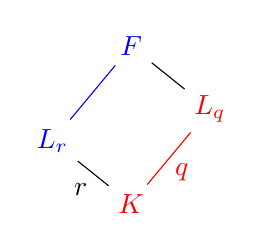
\begin{tikzpicture}

            \node [red] (Q1) at (0,0) {$K$};
            \node [red] (Q2) at (1,1.2) {$L_q$};
            \node [blue] (Q3) at (0,2) {$F$};
            \node [blue] (Q4) at (-1,0.8) {$L_r$};
        
            \draw [red] (Q1)--(Q2) node [pos=0.8, below,inner sep=0.25cm] {$q$};
            \draw (Q1)--(Q4) node [pos=0.9, below,inner sep=0.25cm] {$r$};
            \draw [blue] (Q3)--(Q4);
            \draw (Q2)--(Q3);
        
        \end{tikzpicture}
        \caption[short]{Subfields of a $C_{pq}$-extension}
    \end{figure}

    Again, the result follows immediately from the table and \eqref{eqn_local_contr}.
    
\end{proof}

We are finally ready to prove the main result of this section, from which Theorem \ref{thm_consistent_cyclic} will follow. 

\begin{lemma}\label{lem_Cd_odd}
    Let $d$ be a composite, odd squarefree integer and let $F/K$ be a Galois extension of number fields such that $\Gal(F/K)=C_{d}$. Let $E/\QQ$ be an elliptic curve with semistable reduction at $2$ and $3$ and let $L_k$ be the intermediate fields such that $\Gal(F/L_k)=C_{d/k}$. If 
    $$\Theta_d=\sum_{k\mid d}\mu(k)C_k\in B(C_d),$$
    then $C(\Theta_d)\in\QQss$.
\end{lemma}

\begin{proof}
    Let $n$ be the number of distinct prime numbers dividing $d$, so that $d=p_1\ldots p_n$ for some distinct odd primes $p_i$. We prove this result by induction. The base case for $n=2$ is the content of Lemma \ref{lem_Cpq}. Assume that the result holds for squarefree cyclic Galois extensions with $n-1$ prime factors and consider the two sets of subgroups
    $$\mathcal{A}=\{C_k:p_n\mid k\}\quad\text{and}\quad\mathcal{B}=\{C_k:p_n\nmid k\},$$
    which are clearly a partition of subgroups of $C_d$. Furthermore, the fields $\{F^{C_k}:C_k\in\mathcal{A}\}$ are precisely the intermediate fields of $L_{d/p_n}/K$, while the fields $\{F^{C_k}:C_k\in\mathcal{B}\}$ are the intermediate fields of $F/L_{p_n}$.
    Let 
    $$\Theta_\mathcal{A}=\sum_{H\in\mathcal{A}}\mu(|H|/p_n)H\quad\text{and}\quad\Theta_\mathcal{B}=\sum_{H\in\mathcal{B}}\mu(|H|)H$$
    and we note that
    \begin{equation}\label{eqn_theta}
        \Theta_d=\sum_{k\mid d}\mu(k)C_k=\sum_{p_n\nmid k\mid d}\mu(|C_k|)C_k-\sum_{p_n\mid k\mid d}\mu(|C_k|/p_n)C_k=\Theta_\mathcal{B}-\Theta_\mathcal{A}.
    \end{equation}
    Since $\Gal(L_{d/p_n}/K)=\Gal(F/L_{p_n})=C_{d/p_n}$, it follows from the inductive hypothesis applied to $L_{d/p_n}/K$ and $F/L_{p_n}$ that $C(\Theta_\mathcal{A}),C(\Theta_\mathcal{B})\in\QQss$, and therefore
    $$C(\Theta_d)=\frac{C(\Theta_\mathcal{B})}{C(\Theta_\mathcal{A})}\in\QQss,$$ 
    as desired.
    \begin{figure}[!ht]
        \centering
        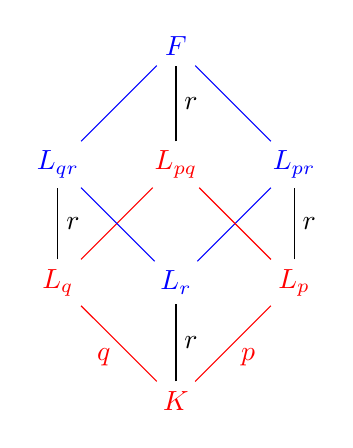
\begin{tikzpicture}

            \node [red] (Q1) at (0,0) {$K$};
            \node [red] (Q2) at (-1.5,1.5) {$L_q$};
            \node [blue] (Q3) at (0,1.5) {$L_r$};
            \node [red] (Q4) at (1.5,1.5) {$L_p$};
            \node [blue] (Q5) at (-1.5,3) {$L_{qr}$};
            \node [red] (Q6) at (0,3) {$L_{pq}$};
            \node [blue] (Q7) at (1.5,3) {$L_{pr}$};
            \node [blue] (Q8) at (0,4.5) {$F$};

            \draw [red] (Q1)--(Q2) node [pos=0.7, below,inner sep=0.25cm] {$q$};
            \draw [red] (Q1)--(Q4) node [pos=0.7, below,inner sep=0.25cm] {$p$};
            \draw (Q1)--(Q3) node [pos=0.5, right,inner sep=0.1cm] {$r$};
            \draw (Q2)--(Q5) node [pos=0.5, right,inner sep=0.1cm] {$r$};
            \draw (Q2)--(Q6) [red];
            \draw (Q3)--(Q5) [blue];
            \draw (Q3)--(Q7) [blue];
            \draw (Q4)--(Q6) [red];
            \draw (Q4)--(Q7) node [pos=0.5, right,inner sep=0.1cm] {$r$};
            \draw (Q5)--(Q8) [blue];
            \draw (Q6)--(Q8) node [pos=0.5, right,inner sep=0.1cm] {$r$};
            \draw (Q7)--(Q8) [blue];
        
        \end{tikzpicture}
        \caption[short]{Partition of $n=3$ into $n=2$. Red fields are in $\mathcal{A}$ while blue fields are in $\mathcal{B}$.}
    \end{figure}
\end{proof}

The proof of Theorem \ref{thm_consistent_cyclic} for odd $d$ is now straightforward.

\begin{proof}[Proof of Theorem \ref{thm_consistent_cyclic} for odd $d$]
    The proof is divided into two cases depending on whether $d$ is the power of a prime or not. Suppose first that $d$ is not, so that $\rad(d)$ is a squarefree \textbf{composite} number. Then $\Theta_d=\sum_{k\mid d}\mu(k)C_k\in B(C_d)$ is the $\psi_d$-relation of a faithful character of $C_d$. The subgroups appearing on $\Theta_d$ are the subgroups of $C_{\rad(d)}$ and therefore by Lemma \ref{lem_Cd_odd} applied to the $C_{\rad(d)}$ extension $F/F^{C_{\rad(d)}}$, it follows that 
    $$C(\Theta_d)\in\QQss,$$ and therefore it is the norm of an element for any quadratic extension of $\QQ$. 

    If $d=q^n$ for some odd prime $q$ and $n\geq1$, then Lemma \ref{lem_relation} shows that $\Theta_d=C_1-C_q$ is the $\psi_d$-relation of a faithful character of $C_d$. Lemma \ref{lem_Cp} applied to the $C_q$ extension $F/F^{C_q}$ proves that 
    $$C(\Theta_d)=\frac{C(C_1)}{C(C_q)}\in N_{\QQ(\sqrt{q^*})/\QQ}(\QQ(\sqrt{q^*})^{\times}).$$ 
    By Lemma \ref{lem_subfields} this is the only quadratic subfield of $\QQ(\zeta_{q^n})$, so the result follows.
\end{proof}

 
\subsubsection{Even Cyclic Extensions}
More care is required to prove Theorem \ref{thm_consistent_cyclic} for even $d$. This difficulty mainly lies in the case when $d$ is only divisible by one odd prime $q$. Consequently, we break down the proof into three distinct cases according to the number of odd prime divisors of $d$. If $d$ has more than one odd prime divisor, then the result follows without much work from Lemma \ref{lem_Cd_odd}, so we prove this first.

\begin{proof}[Proof of Theorem \ref{thm_consistent_cyclic} for even $d$ with more than one odd prime divisor]
    By Remark \ref{rem_radical}, recall that the subgroups present in $\Theta_d$ are precisely those such that $C_k\leq C_{\rad(d)}$, and so following a similar idea to Lemma \ref{lem_Cd_odd}, we define
    $$\mathcal{A}=\{C_k :2\mid k\mid\rad(d)\}\quad\text{and}\quad\mathcal{B}=\{C_k:2\nmid k\mid\rad(d)\},$$
    together with
    $$\Theta_\mathcal{A}=\sum_{H\in\mathcal{A}}\mu(|H|/2)H\quad\text{and}\quad\Theta_\mathcal{B}=\sum_{H\in\mathcal{B}}\mu(|H|)H. $$ 
    For each $k\mid d$, let $L_k=F^{C_{d/k}}$ be the unique subfield of degree $k$ over $K$. The fields $\{F^{C_k}:C_k\in\mathcal{A}\}$ are the intermediate fields of $L_{d/2}/L_{d/\rad(d)}$ and the fields $\{F^{C_k}:C_k\in\mathcal{A}\}$ are the intermediate fields of $F/L_{2d/\rad(d)}$. However, note that 
    $$\Gal(L_{d/2}/L_{d/\rad(d)})=\Gal(F/L_{2d/\rad(d)})=C_{\rad(d)/2},$$
    and by assumption $\rad(d)/2$ is an odd number with more than one prime factor. Then Lemma \ref{lem_subfields} applied to $L_{d/2}/L_{d/\rad(d)}$ and $F/L_{2d/\rad(d)}$ gives $\Theta_\mathcal{A},\Theta_\mathcal{B}\in\QQss$. The calculation in \eqref{eqn_theta} shows that $\Theta_d=\Theta_\mathcal{B}-\Theta_\mathcal{A}$ and therefore 
    $$C(\Theta_d)=\frac{C(\Theta_\mathcal{B})}{C(\Theta_\mathcal{A})}\in\QQss$$
    is the norm of any quadratic extension.
\end{proof}

If $d$ has no odd primes factors, then $d=2^l$ for some $l\geq1$. In that case, we assume in Theorem \ref{thm_consistent_cyclic} that $E$ is semistable, and the proof under this assumption is short. 

\begin{proof}[Proof of Theorem \ref{thm_consistent_cyclic} for $d=2^l$ and semistable $E$]

    If $l=1$, then $\QQ(\zeta_2)=\QQ$, and there is nothing to prove, so assume that $l\geq2$. If $\Gal(F/\QQ)=C_{2^l}$, then 
    $$C(\Theta_d)=\frac{C(C_1)}{C(C_2)}=\frac{C_{E/F}}{C_{E/L_{2^{l-1}}}},$$
    and $F/L_{2^{l-1}}$ is a $C_2$ extension. Importantly, we note that Table \ref{table_Cp} also applies for $q=2$, and therefore $\Cp(\Theta_d)$ is a rational square up to factors of $2$ for any prime $\pp$ of $L_{2^{l-1}}$. Lemma \ref{lem_subfields} shows that the only subfields of $\QQ(\zeta_{2^l})$ are $\QQ(i),\QQ(\sqrt{2})$ and $\QQ(\sqrt{-2})$, and since
    $$2=\Norm_{\QQ(i)}(1+i)=\Norm_{\QQ(\sqrt{-2})}(2)=\Norm_{\QQ(\sqrt{2})}(2+\sqrt{2}),$$
    it follows that $\Cp(\Theta_d)$ is a norm from every quadratic subfield of $\QQ(\zeta_{2^l})$, and the result follows.
\end{proof}

The remaining of this section is therefore devoted to the case when $d$ is divisible by one odd prime $q$, so $d=2^mq^n$. 
%When $d$ has this form, then $\Theta_d=C_1-C_2-C_q+C_{2q}$ and therefore fix $\Theta_d$ to have this expression for the remaining of this section. 
Recall that the quadratic subfields of $\QQ(\zeta_{2^mq^n})$ depend on whether $m=1$, $m=2$ or $m\geq 3$. Consequently, we prove three results that will be essential to prove the general version of each different case. The first covers the case $m=1$.

\begin{lemma}\label{lem_C2p}
    Let $q$ be an odd prime and let $F/K$ be a Galois extension of number fields such that $\Gal(F/K)=C_{2q}$ and let $L_k=F^{C_{2q/k}}$ be the intermediate fields such that $[L_k:K]=k$. Let $E/\QQ$ be an elliptic curve and let $\Theta_{2q}=C_{2q}-C_q-C_2+C_1\in B(C_{2q})$. Then
    $$C(\Theta_{2q})=\frac{C_{E/F}C_{E/K}}{C_{E/L_2}C_{E/L_q}}$$
    is a norm from $\QQ(\sqrt{q^*})$.
\end{lemma}

\begin{proof}
    Similarly to the proofs of Lemma \ref{lem_Cp} and \ref{lem_Cpq}, let $\pp$ be a prime in $K$ and assume that $\Delta_E=\Delta_{E,\pp}^{\min}$. The splitting behaviour of a prime $\pp$ in $K$ is again determined by $e_\pp$ and $f_\pp$ and therefore if $\pp$ has multiplicative reduction $\Dp(\Theta_{2q})=1$ and the following table records $\Tp(\Theta_{2q})$.

    \begin{table}[!ht]
        \centering
        \begin{tabular}{|l|l|l|l|l|l|l|}
        \hline
        $e_\pp$ & $f_\pp$  & $\Tp(C_{2q})$ & $\Tp(C_2)$ & $\Tp(C_q)$ & $\Tp(C_1)$ & $\Tp(\Theta_{2q})$ \\ \hline
        $1$ & $1$ & $n;\tilde{n}$ & $n^q;\tilde{n}^q$ & $n^2;\tilde{n}^2$ & $n^{2q};\tilde{n}^{2q}$ & $\square$ \\ \hline
        $1$ & $q$ & $n;\tilde{n}$ & $n;\tilde{n}$ & $n^2;\tilde{n}^2$ & $n^2;\tilde{n}^2$ & $\square$ \\ \hline
        $1$ & $2$ & $n;\tilde{n}$ & $n^q;\tilde{n}^q$ & $n;n$ & $n^q;n^q$ & $\square$ \\ \hline
        $1$ & $2q$ & $n;\tilde{n}$ & $n;\tilde{n}$ & $n;n$ & $n;n$ & $\square$ \\ \hline
        $q$ & $1$ & $n;\tilde{n}$ & $qn;\tilde{n}$ & $n^2;\tilde{n}^2$ & $q^2n^2;\tilde{n}^2$ & $q\square;\square$ \\ \hline
        $q$ & $2$ & $n;\tilde{n}$ & $qn;\tilde{n}$ & $n;n$ & $qn;n$ & $\square$ \\ \hline
        $2$ & $1$ & $n;\tilde{n}$ & $n^q;\tilde{n}^q$ & $2n;1$ & $2^qn^q;1^q$ & $\square$ \\ \hline
        $2$ & $q$ & $n;\tilde{n}$ & $n;\tilde{n}$ & $2n;1$ & $2n;1$ & $\square$ \\ \hline
        $2q$ & $1$ & $n;\tilde{n}$ & $qn;\tilde{n}$ & $2n;1$ & $2qn;1$ & $\square$ \\ \hline
        \end{tabular}
        \caption{Contribution of multiplicative reduction primes in a $C_{2q}$ extension.}
    \end{table}

    Since $q$ is a norm from $\QQ(\sqrt{q^*})$, then $\Tp(\Theta_{2q})$ is also a norm. Now assume that $\pp$ has additive reduction and let $p\ZZ=\pp\cap\QQ$. We first consider the contribution of the Tamagawa numbers. Note that $L_q/K$ and $F/L_2$ are $C_q$ extensions and therefore $\Tp(\Theta_{2q})\in\QQss$ if $q\neq 3$ and a square up to factors of $3$ if $q=3$. In either case, $\Tp(\Theta_{2q})$ is a norm from $\QQ(\sqrt{q^*})$.

    Finally, to compute $\Dp(\Theta_{2q})$, let $n=\nu_\pp(\Delta_{E,\pp}^{\min})$ and note that all terms cancel unless $\pp$ ramifies in $F$. If $e_\pp=2$, then
    \begin{equation}\label{eqn_ep=2}
        \Dp(C_{2q})=\Dp(C_2)=1,\quad \Dp(C_q)=N(\pp)^{\floor{\frac{2n}{12}}}\quad\text{and}\quad \Dp(C_1)=N(\pp)^{q\floor{\frac{2n}{12}}},
    \end{equation}
    and therefore $D(\Theta_{2q})=N(\pp)^{(q-1)\floor{n/6}}\in\QQss$, a rational square. If $q\mid e_\pp$, then $q\mid N(\pp)-1$ by Proposition \ref{prop_totally_ramified}, and the reasoning is now identical to Lemma \ref{lem_Cp}. Write $N(\pp)=p^s$ for some $s\geq1$ and note that $\Dp(\Theta_{2q})\in\QQss$ if $s$ is even. Hence, we assume that $s$ is odd. In this case, $p=q$ if $(L_q)_\fP/K_\pp$ is wildly ramified and $p$ splits in $\QQ(q^*)$ if $(L_q)_\fP/K_\pp$ is tamely ramified. In either case, by Corollaries \ref{p-norm} and \ref{cor_psplit_pnorm}, $p$ is a norm from $\QQ(\sqrt{q^*})$, and hence so is $\Dp(\Theta_{2q})$.
    The result follows again from \eqref{eqn_local_contr}.
\end{proof}

Following this, we state and prove the analogous result for $m=2$.

\begin{lemma}\label{lem_C4p}
    Let $q$ be an odd prime and let $F/K$ be a Galois extension of number fields such that $\Gal(F/K)=C_{4q}$ and let $L_k=F^{C_{4q/k}}$ be the intermediate fields such that $[L_k:K]=k$. Let $E/\QQ$ be an elliptic curve with semistable reduction at $2$ and $3$ and let $\Theta_{4q}=C_1-C_2-C_q+C_{2q}$. Then 
    $$C(\Theta_{4q})=\frac{C_{E/F}C_{E/L_2}}{C_{E/L_4}C_{E/L_{2q}}}$$
    is a norm from $\QQ(i),\QQ(\sqrt{q})$ and $\QQ(\sqrt{-q})$. Moreover, $\Tp(\Theta_{4q})\in\QQss$ for any prime $\pp$ in $K$, and $\Dp(\Theta_{4q})\in\QQss$ unless $E$ has additive reduction at $\pp$ and $\pp$ is totally ramified in $F/K$.
\end{lemma}

\begin{proof}
    All fields appearing in the product are intermediate fields of $F/L_2$, and $\Gal(F/L_2)=C_{2q}$. Let $\pp$ be a prime in $K$, let $\bar\pp\mid\pp$ be a prime above $\pp$ in $L_2$ and let $p\ZZ=\pp\cap\QQ$. Assume also that $\Delta_E=\Delta_{E,\pp}^{\min}$. Lemma \ref{lem_C2p} shows that if $E$ has multiplicative reduction over $\bar\pp$, $C_{\fP\mid\bar\pp}(\Theta_{4q})\in\QQss$ unless $e_{\bar\pp}=q$ and $f_{\bar\pp}=1$ over $F$. When this holds, $\bar\pp$ ramifies in $L_{2q}/L_2$ and is split in $L_4/L_2$, and this forces $\pp$ to split in $L_2/K$ too. Hence, $\pp=\bar\pp\bar\pp'$ for two \textbf{distinct} primes in $K$ that have the same local behaviour and therefore $\Cp(\Theta_{4q})=C_{\fP\mid\bar\pp}(\Theta_{4q})C_{\fP\mid\bar\pp'}(\Theta_{4q})=C_{\fP\mid\bar\pp}(\Theta_{4q})^2\in\QQss$, as desired.

    \begin{figure}[!ht]
        \centering
        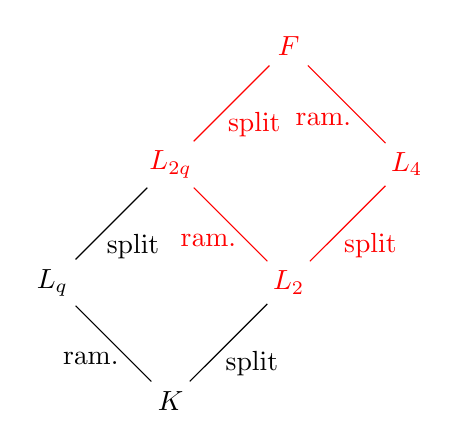
\begin{tikzpicture}

            \node (Q1) at (0,0) {$K$};
            \node (Q2) at (-1.5,1.5) {$L_q$};
            \node [red] (Q3) at (3,3) {$L_4$};
            \node [red] (Q4) at (1.5,1.5) {$L_2$};
            \node [red] (Q5) at (1.5,4.5) {$F$};
            \node [red] (Q6) at (0,3) {$L_{2q}$};
            

            \draw (Q1)--(Q2) node [pos=0.8, below,inner sep=0.4cm] {ram.};
            \draw (Q1)--(Q4) node [pos=0.8, below,inner sep=0.4cm] {split};
            \draw (Q2)--(Q6) node [pos=0.8, below,inner sep=0.4cm] {split};
            \draw [red] (Q3)--(Q5) node [pos=0.8, below,inner sep=0.4cm] {ram.};
            \draw [red] (Q4)--(Q6) node [pos=0.8, below,inner sep=0.4cm] {ram.};
            \draw [red] (Q6)--(Q5) node [pos=0.8, below,inner sep=0.4cm] {split};
            \draw [red] (Q4)--(Q3) node [pos=0.8, below,inner sep=0.4cm] {split};
        \end{tikzpicture}
        \caption[short]{\centering Field diagram for a $C_{4q}$ extension, together with the splitting\newline behaviour of a prime $\pp$ in $L_2$ with $e_\pp=q$ and $f_\pp=1$ over $F$.}
    \end{figure}

    Assume now that $E$ has additive reduction over $\bar\pp$. When $q=3$, controlling the Tamagawa numbers is lengthy, so we leave it for the end. We calculate first $\Dp(\Theta_{4q})$, which is $1$ unless $\bar\pp$ ramifies in $L/F_2$ (equivalently, $\pp$ ramifies in $L/K$). If $\pp$ is inert in $L_2/K$, then $N(\bar{\pp})\in\QQss$ and hence the size of all residues fields above $\pp$ are also squares and consequently $\Dp(\Theta_{4q})\in\QQss$ using Lemma \ref{lem_Dterms}. If $\pp=\bar\pp\bar\pp'$ splits, then $D_{\fP\mid\bar\fp}(\Theta_{4q})=D_{\fP\mid\bar\fp'}(\Theta_{4q})$, and therefore $\Dp(\Theta_{4_q})\in\QQss$ too. Finally, assume that $\pp=\bar\pp^2$ ramifies in $L_2/K$, which implies that $\bar\fp$ also ramifies in $L_4/L_2$. On the other hand, if $\bar\pp$ is unramified at $L_{2q}/L_2$, \eqref{eqn_ep=2} during the proof of Lemma \ref{lem_C2p} shows that $\Dp(\Theta_{4q})\in\QQss$ too. 

    We are therefore left with the case where $\pp$ is totally ramified in $F/K$, and Proposition \ref{prop_totally_ramified} implies that $4q\mid N(\pp)-1$. If we let $n=\nu_{\pp}(\Delta_{E,\pp}^{\min})$, Lemma \ref{lem_Dterms} implies that 
    \begin{equation*}\label{eqn_DtermsC4p}
        \Dp(\Theta_{4q})=N(\pp)^{\floor{\frac{n}{6}}-\floor{\frac{n}{3}}-\floor{\frac{qn}{6}}+\floor{\frac{qn}{3}}}.
    \end{equation*}
    Again, the parity of the expression only depends on $q,n\pmod{12}$. One can easily check that for $n\in\{2,3,4,6,8,9,10\}$ and $q\in\{1,5,7,11\}$, the above expression is a square unless $q\equiv 3\pmod{4}$ and $n$ is odd, so we assume this is the case. Write $N(\pp)=p^s$ for some $s\geq1$, which satisfies $p^s\equiv1\pmod{4q}$. If $s$ is even, then $\Dp(\Theta_{4q})\in\QQss$, so assume that $s$ is odd. Since $p^s\equiv1\pmod{4}$, this implies that $p\equiv1\pmod{4}$ and hence $p$ is a norm from $\QQ(i)$, which implies that $\Dp(\Theta_{4q})$ is a norm from $\QQ(i)$ too. Furthermore, the fact that $p^s\equiv1\pmod{4q}$ implies that
    $$\left(\frac{-q}{p}\right)=\left(\frac{q}{p}\right)=\left(\frac{p}{q}\right)=\left(\frac{p^s}{q}\right)=1,$$
    and therefore $p$ splits both in $\QQ(\sqrt{q})$ and $\QQ(\sqrt{-q})$. Since $q\equiv3\pmod{4}$, both fields have odd class number (Theorem \ref{thm_class_number}), and hence $p$ and $\Dp(\Theta_{4q})$ are norms from $\QQ(\sqrt{q})$ and $\QQ(\sqrt{-q})$ as desired. 

    Finally, we discuss Tamagawa numbers. Note that $L_{2q}/L_2$ and $F/L_4$ are $C_q$ extensions and therefore by Lemma \ref{lem_Cp} it follows that $\Dp(\Theta_{4q})\in\QQss$ if $q\neq3$. If $q=3$, it is also the case that $\Dp(\Theta_{4q})\in\QQss$, but more work is required. We prove this as a separate lemma, from which the result follows.    
\end{proof}

\begin{lemma}
    Let $L/K$ be a Galois extension of number fields with $\Gal(L/K)=C_{12}$ and let $L_k=F^{C_{12/k}}$ be the intermediate fields such that $[L_k:K]=k$. Let $E/\QQ$ be an elliptic curve and let $\pp$ be a prime in $K$ not dividing $2$ or $3$ such that $E$ has potentially good reduction at $\pp$. If $\Theta_{12}=C_1-C_2-C_3+C_6\in B(C_{12})$, then $$\Tp(\Theta_{12})=\frac{\Tp(E/F)\Tp(E/L_2)}{\Tp(E/L_6)\Tp(E/L_4)}\in\QQss.$$
\end{lemma}
\begin{proof}
    Let $\bar\pp$ be a prime in $L_2$ above $\pp$ and let $n=\nu_{\bar\pp}(\Delta_{E,\bar\pp}^{\min})$ be the minimal discriminant of $E$ at $\bar\pp$. If $\pp$ is unramified in $L_3/K$, then so is $\bar\pp$ in $L_6/L_2$ and the primes above them in $F/L_4$. From Lemma \ref{lem_Cp}, we know that that the product of Tamagawa numbers in unramified $C_3$ extensions is a square, so assume that $\pp$ ramifies in $L_3/K$.

    The proof is now divided in three cases, depending on the splitting behaviour of $\pp$ in $L_2$. If $\pp$ splits in $L_2/K$, then $\pp=\bar\pp\bar\pp'$ where $\bar\pp$ and $\bar\pp'$ have the same local behaviour. Therefore, $T_{\fP\mid\pp}(\Theta_{12})=T_{\fP\mid\bar\pp}(\Theta_{12})T_{\fP\mid\bar\pp'}(\Theta_{12})\in\QQss$. 
    
    Next, suppose that $\pp$ is inert in $L_2/K$, which implies that $\bar\pp$ is either inert or ramified in $L_4/L_2$. Let $\fP$ be the prime in $L_4$ above $\bar\pp$. If $\bar\pp$ is inert in $L_4/L_2$, then the valuation of the minimal discriminant of $E$ at $\fP$ is also $n$ and the splitting behaviour of $\bar\pp$ in $L_6/L_2$ coincides with the splitting behaviour of $\fP$ in $F/L_4$. Hence, 
    $$\frac{\Tp(E/F)}{\Tp(E/L_4)}=\frac{\Tp(E/L_6)}{\Tp(E/L_2)},$$
    and therefore $\Tp(\Theta_{12})=1$. The case where $\bar\pp$ is ramified in $L_4/L_2$ is more subtle. We have already seen that in ramified $C_3$ extensions we cannot obtain factors of $2$. Upon inspection of Lemma \ref{lem_add_tam}, one can easily show that the Tamagawa numbers cancel out if $\gcd(n,12)\in\{3,4,6,12\}$, so we only need to consider the case $\gcd(n,12)=2$. Since $\Gal((L_4)_\fP/K_\pp)=C_4$ and $e_{\fP\mid\pp}=f_{\fP\mid\pp}=2$, Lemma \ref{lem_notthree} shows that $\sqrt{B}\not\in F_{\fP}$ and therefore $c_\fP(E/F)=1$, which imples that $\Dp(\Theta_{12})\in\QQss$.

    Finally, assume that $\pp$ ramifies in $L_2/K$ so that $\pp=\bar\pp^2$. This immediately implies that $\bar\pp$ also ramifies in $L_4/L_2$, and therefore $\pp$ is totally ramified in $F/K$. As mentioned above, the Tamagawa numbers cancel unless $\gcd(n,12)=2$. However, recall that $E$ has potentially good reduction at $\pp$, and since $\pp=\bar\pp^2$ ramifies, then the valuation of the minimal discriminant at $\pp$ is $n/2$ or $(n+12)/2$. But then $\gcd(\nu_\pp(\Delta_{E,\pp}^{\min}),12)=\gcd(n/2,12)=1$, a contradiction. Hence, $\Tp(\Theta_{12})\in\QQss$ as desired.
\end{proof}

Finally, we state and prove the last result, from which the case $m\geq3$ follows easily. One needs to check that the product of local factors is the norm of many quadratic subfields; thankfully, Lemma \ref{lem_C4p} has done most of work required.

\begin{lemma}\label{lem_C8p}
    Let $q$ be an odd prime and let $F/K$ be a Galois extension of number fields such that $\Gal(F/K)=C_{8q}$ and let $L_k=F^{C_{8q/k}}$ be the intermediate fields such that $[L_k:K]=k$. Let $E/\QQ$ be an elliptic curve with semistable reduction at $2$ and $3$ and let $\Theta_{8q}=C_1-C_2-C_q+C_{2q}$. Then 
    $$C(\Theta_{8q})=\frac{C_{E/F}C_{E/L_4}}{C_{E/L_8}C_{E/L_{4q}}}\in\QQss.$$
    %is a norm from $\QQ(\sqrt{D})$ for each $D\in\{-1,\pm2,\pm q,\pm 2q\}$.
\end{lemma}

\begin{proof}
    We prove the result locally for all primes in $L_2$, and note $\Gal(F/L_2)=4q$. Let $\bar\pp$ and assume that $\Delta_E=\Delta_{E,\bar\pp}^{\min}$. Since the relation $\Theta_{4q}=C_1-C_2-C_q+C_{2q}\in B(C_{4q})$ has the same fixed fields as $\Theta_{8q}$, by Lemma \ref{lem_C4p}, we know that $\Tpb(\Theta_{8q})\in\QQss$ for any $\bar\pp$ and $\Dpb(\Theta_{8q})\in\QQss$ too unless $\bar\pp$ is totally ramified in $F/L_2$ and $E$ has potentially good reduction at $\bar\pp$, so assume this is the case. If $\pp=\bar\pp\cap K$, then it also follows that $\pp$ is totally ramified in $F/K$ and $E$ has potentially good reduction at $\pp$. If $n=\nu_{\bar\pp}(\Delta_{E,\bar\pp}^{\min})$, then recall from Lemma \ref{lem_C4p} that 
    $$\Dpb(\Theta_{8q})=N(\bar\pp)^{\floor{\frac{n}{6}}-\floor{\frac{n}{3}}-\floor{\frac{qn}{6}}+\floor{\frac{qn}{3}}},$$
    and that the exponent is even unless $n$ is odd and $q\equiv 3\pmod{4}$. However, $\pp=\bar\pp^2$ is ramified in $L_2/K$ and therefore $n\equiv 2\nu_\pp(\Delta_{E,\pp}^{\min})\pmod{12}$. That is, $n$ is even and therefore $\Dpb(\Theta_{8q})\in\QQss$ as desired.
\end{proof}
%%% THIS IS ALL PROBABLY NOT NEEDED NOW
%Again, $\Dp(\Theta_{8q})$ does not change up to squares if $\Delta_{E}$ is reescaled so assume that $\Delta_{E}=\Delta_{E,\pp}^{\min}$. Under these assumptions, $\Dpb(\Theta_{8q})=\Dp(\Theta_{8q})$ is a power of $N(\pp)=N(\bar\pp)=p^s$ for some rational prime $p$ and $s\geq1$. If $s$ is even, then $\Dpb(\Theta_{8q})\in\QQss$, so assume that $s$ is odd. In addition, by Proposition \ref{prop_totally_ramified}, it follows that $p^s\equiv 1\pmod{8q}$. Since $s$ is odd and $(\ZZ/8\ZZ)^*=C_2\times C_2$, it follows that $p\equiv 1\pmod{8}$ and therefore
%\begin{equation}\label{eqn_psplitsin2}
%    \left(\frac{-1}{p}\right)=\left(\frac{2}{p}\right)=\left(\frac{-2}{p}\right)=1.
%\end{equation}
%Furthermore, since $p^s\equiv1\pmod{8s}$ and $s$ is odd, then 
%\begin{equation}\label{eqn_psplitsinq}
%    \left(\frac{-q}{p}\right)=\left(\frac{q}{p}\right)=\left(\frac{p}{q}\right)=1.
%\end{equation}
%Combining \eqref{eqn_psplitsin2} and \eqref{eqn_psplitsinq} together with multiplicativity of the Legendre symbol, it follows that $p$ splits in every quadratic subfield $\QQ(\sqrt{D})$ for $D\in\{-1,\pm2,\pm q,\pm2q\}$.


We are now ready to prove the remaining case of Theorem \ref{thm_consistent_cyclic}.

\begin{proof}[Proof of Theorem \ref{thm_consistent_cyclic} for $d$ even and with one odd prime factor.]
    In this case, write $d=2^mq^n$ for $n,m\geq 1$ and note that $\Theta_{d}=C_1-C_2-C_q+C_{2q}$ is the $\psi_d$-relation of a faithful character of $C_d$. If $m=1$, Lemma \ref{lem_C2p} applied to the $C_{2q}$ extension $F/F^{C_{2q}}$ shows that $C(\Theta_d)$ is a norm from $\QQ(\sqrt{q^*})$, which is the only subfield of $\QQ(\zeta_{2q^n})$ by Lemma \ref{lem_subfields}. If $m=2$, then Lemma \ref{lem_C4p} applied to the $C_{4q}$ extension $F/F^{C_{4q}}$ shows that $C(\Theta_{d})$ is a norm from $\QQ(i),\QQ(\sqrt{q})$ and $\QQ(\sqrt{-q})$, which are all quadratic subfields of $\QQ(\zeta_{4q^n})$. Finally, if $m\geq3$, Lemma \ref{lem_C8p} applied to $F/F^{C_{8q}}$ shows that $C(\Theta_{8q})\in\QQss$, which is the norm from any quadratic subfield. The result follows.
\end{proof}

